% A1a report: Slot filling on ATIS, CRF vs BiLSTM
% Numbers and tables come from report/make_tables.py (numbers.tex, tables/*.tex).
% Rerun that script after any retraining; never type a number by hand.
% Search for \todo to find everything that still needs your writing.
\documentclass[10pt,twocolumn]{article}
\usepackage[letterpaper,margin=0.7in,columnsep=0.25in]{geometry}
\usepackage[compact]{titlesec}
\titlespacing*{\section}{0pt}{1.0ex plus .3ex}{0.6ex}
\usepackage[T1]{fontenc}
\usepackage{lmodern}
\usepackage{microtype}
\usepackage{graphicx}
\usepackage{booktabs}
\usepackage{tabularx}
\usepackage{xcolor}
\usepackage{caption}
\usepackage{enumitem}
\usepackage{float}
\usepackage[hidelinks]{hyperref}
\captionsetup{font=small,labelfont=bf,skip=4pt}
\setlist{nosep,leftmargin=1.2em}
\setlength{\parskip}{3pt}
\setlength{\parindent}{0pt}
% Let two table* floats share the top of a page (Tables 1 and 5).
\renewcommand{\dbltopfraction}{0.9}
\setcounter{dbltopnumber}{2}

% Placeholder box for your writing. Set \showtodosfalse to hide them all.
\newif\ifshowtodos \showtodosfalse % set to \showtodostrue to show TODO boxes
\newcommand{\todo}[1]{\ifshowtodos{\color{red!70!black}\textbf{[TODO:} #1\textbf{]}}\fi}

% Slot names with underscores, e.g. \slot{arrive_time.time}
\newcommand{\slot}[1]{\texttt{\detokenize{#1}}}

% Auto-generated by report/make_tables.py -- do not edit by hand.
\newcommand{\crfRoleIdentity}{336}
\newcommand{\crfWrongTypeIdentity}{348}
\newcommand{\crfRoleCtxOne}{101}
\newcommand{\crfRoleFull}{60}
\newcommand{\crfDevFiveFull}{0.853}
\newcommand{\crfDevFiveNoGaz}{0.835}
\newcommand{\crfDevFiveNoAffix}{0.834}
\newcommand{\crfDevFiveNoOrtho}{0.851}
\newcommand{\crfDevFiveIdentity}{0.662}
\newcommand{\crfDevFiveNoCtx}{0.696}
\newcommand{\crfDevIdentity}{0.778}
\newcommand{\crfDevCtxOne}{0.928}
\newcommand{\crfDevNoGaz}{0.951}
\newcommand{\crfDevNoCtx}{0.783}
\newcommand{\crfDevFull}{0.954}
\newcommand{\crfTestFive}{0.847}
\newcommand{\lstmTestFive}{0.819}
\newcommand{\smTestFive}{0.801}
\newcommand{\crfDevFiveFrac}{0.853}
\newcommand{\lstmDevFive}{0.848}
\newcommand{\smDevFive}{0.825}
\newcommand{\oldLstmTestFive}{0.798}
\newcommand{\oldLstmDevFive}{0.835}
\newcommand{\nSentFive}{224}
\newcommand{\crfTestTen}{0.887}
\newcommand{\lstmTestTen}{0.882}
\newcommand{\smTestTen}{0.865}
\newcommand{\crfDevTenFrac}{0.891}
\newcommand{\lstmDevTen}{0.899}
\newcommand{\smDevTen}{0.882}
\newcommand{\oldLstmTestTen}{0.859}
\newcommand{\oldLstmDevTen}{0.875}
\newcommand{\nSentTen}{448}
\newcommand{\crfTestTwentyFive}{0.905}
\newcommand{\lstmTestTwentyFive}{0.920}
\newcommand{\smTestTwentyFive}{0.917}
\newcommand{\crfDevTwentyFiveFrac}{0.925}
\newcommand{\lstmDevTwentyFive}{0.949}
\newcommand{\smDevTwentyFive}{0.943}
\newcommand{\oldLstmTestTwentyFive}{0.913}
\newcommand{\oldLstmDevTwentyFive}{0.935}
\newcommand{\nSentTwentyFive}{1,120}
\newcommand{\crfTestFull}{0.936}
\newcommand{\lstmTestFull}{0.952}
\newcommand{\smTestFull}{0.949}
\newcommand{\crfDevFullFrac}{0.954}
\newcommand{\lstmDevFull}{0.979}
\newcommand{\smDevFull}{0.974}
\newcommand{\oldLstmTestFull}{0.951}
\newcommand{\oldLstmDevFull}{0.974}
\newcommand{\nSentFull}{4,478}
\newcommand{\nCrfWrongOnly}{53}
\newcommand{\nLstmWrongOnly}{29}
\newcommand{\nBothWrong}{87}
\newcommand{\nBothRight}{724}
\newcommand{\oovSpans}{50}
\newcommand{\crfOovRecall}{0.540}
\newcommand{\lstmOovRecall}{0.620}


\title{\vspace{-3em}A1a: Slot Filling on ATIS with a CRF and a BiLSTM}
\author{Michael Incorvaia} % check name
\date{September 2026}

\begin{document}
\maketitle
\vspace{-1.5em}

% =====================================================================
\section{Setup}
% Facts about what was built. Edit into your own voice.
ATIS slot filling (4,478 / 500 / 893, 120 slots), strict span F1, every choice made on dev.
The CRF (\texttt{sklearn-crfsuite}, $c_1{=}c_2{=}0.1$) uses word identity, affixes, shape,
a $\pm1$ template with bigrams, lower-cased words at $\pm2$, and gazetteers plus a time regex
(test \crfTestFull).
The BiLSTM is a 2-layer network with random 100-d embeddings and a handwritten CRF layer,
trained at constant lr $10^{-3}$ (test \lstmTestFull); a softmax head is the ablation.
Part~C uses the fixed subsets of \nSentFive, \nSentTen, \nSentTwentyFive, and \nSentFull\ sentences.

\todo{Optional 1--2 sentences: anything else about your design choices.}

% =====================================================================
\section{Part A: CRF feature engineering}
\begin{table*}[t]
\centering\small
\caption{CRF feature log (last column: same features trained on the 5\% subset). Top block adds feature groups
cumulatively; bottom block removes one group from the full set.}
\label{tab:ablation}
\begin{tabular}{@{}lrrrrr@{}}
\toprule
 & \multicolumn{4}{c}{Trained on 100\% (4,478 sent.)} & 5\% (224) \\
\cmidrule(lr){2-5}\cmidrule(l){6-6}
Feature set & \#feats & Dev F1 & Test F1 & Role errs & Dev F1 \\
\midrule
word identity only (current token) & 2,966 & 0.778 & 0.776 & 336 & 0.662 \\
\quad + prefixes/suffixes (1--3 chars) & 7,338 & 0.783 & 0.771 & 336 & 0.678 \\
\quad + casing, digit, shape, length & 8,270 & 0.782 & 0.776 & 337 & 0.675 \\
\quad + all of the above for tokens $\pm1$, bigrams & 20,082 & 0.928 & 0.921 & 101 & 0.832 \\
\quad + lower-cased words at $\pm2$ & 19,922 & 0.951 & 0.933 & 60 & 0.835 \\
\quad + gazetteers / time regex (\textbf{submitted}) & 18,596 & \textbf{0.954} & 0.936 & 60 & \textbf{0.853} \\
\midrule
full $-$ gazetteers & 19,922 & 0.951 & 0.933 & 60 & 0.835 \\
full $-$ affixes & 11,919 & 0.953 & 0.935 & 60 & 0.834 \\
full $-$ orthographic & 16,946 & 0.953 & 0.934 & 61 & 0.851 \\
full $-$ all context & 8,065 & 0.783 & 0.776 & 335 & 0.696 \\
\bottomrule
\end{tabular}
\par\vspace{3pt}\parbox{0.86\linewidth}{\scriptsize \#feats = state features with nonzero weight after training; the L1 penalty ($c_1{=}0.1$) prunes features made redundant by others, so the count can drop when a group is added. Role errs = dev spans with the right boundaries and the right slot but the wrong role (e.g.\ \texttt{toloc} vs \texttt{fromloc}), out of 1,709 gold spans; -- = not measured.}

\end{table*}

\todo{Interpret the feature log. Which groups matter and why, in terms of what
information each one gives the model? Facts to work from: identity only
\crfDevIdentity; adding $\pm1$ context gives \crfDevCtxOne; removing all context
drops the full model from \crfDevFull\ to \crfDevNoCtx; removing gazetteers gives
\crfDevNoGaz. Note every gazetteer entry also appears in the training data.}

Word identity alone (the surface form and its lower-cased form) is a dev F1 of
\crfDevIdentity\ (0.776 test). On ATIS many strings are nearly unambiguous, so a
memorized word-to-slot map already covers the easy spans. Prefixes and suffixes,
then casing, digit, shape, and length, move dev F1 only to 0.783 and then 0.782.
Those groups describe the form of the current token. On the 5\% subset they help
a little: identity alone is \crfDevFiveIdentity\ and affixes raise it to 0.678.
They do not choose a role. Role errors (right boundaries, right slot, wrong role,
as in \slot{toloc.city_name} versus \slot{fromloc.city_name}) are
\crfRoleIdentity\ with identity alone and 337 once orthography is added. The
affix row was not measured. Form features leave the from/to and depart/arrive
decision where they found it.

The score arrives with context. The $\pm1$ template and bigrams raise dev F1
from 0.782 to \crfDevCtxOne\ and cut role errors from 337 to \crfRoleCtxOne,
because the preposition in ``from Boston'' versus ``to Boston'' is what chooses
the role. The next row adds the lower-cased word at $\pm2$. Case-folding of the
current token is already in the identity group. Dev F1 moves from \crfDevCtxOne\
to \crfDevNoGaz, which is enough to see a verb two tokens from a time
(``leaving after noon''). Gazetteers and the time regex then reach \crfDevFull,
and role errors reach \crfRoleFull. Every list entry already occurs in the full
training set, so those features barely move full-data F1 (bottom block of
Table~\ref{tab:ablation}). On \nSentFive\ sentences the missing list items are 13 of 15 airport codes,
11 of 23 airline words, and 10 of 19 day words. Three of the 34 cities are
missing. Removing the lists costs \crfDevFiveFull\ down to \crfDevFiveNoGaz.
Removing context returns the model to \crfDevNoCtx.

% =====================================================================
\section{Part C: Data efficiency}
% Queued here, while page 1 is still being built, so this table* can sit
% with Table 1 at the top of page 2, ahead of the Part D diagnoses.
\begin{table*}[t]
\centering\small
\caption{Ten test failures. Bold = disputed tokens; $^\dagger$ = token never seen in
training. ``Wrong'' says which model errs. Index in parentheses is the test line.}
\label{tab:examples}
{\footnotesize\begin{tabularx}{\linewidth}{@{}l l X@{}}
\toprule
\# & Wrong & Utterance, then the disputed spans (G = gold, C = CRF, L = BiLSTM-CRF) \\
\midrule
D1 (176) & CRF & what meals are available on dl 468$^{\dagger}$ which al$^{\dagger}$ arrives in san francisco at \textbf{950}$^{\dagger}$ \textbf{am} \newline {\footnotesize G: \texttt{arrive\_time.time}=950 am \quad C: \texttt{depart\_time.time}=950 am \quad L: \texttt{arrive\_time.time}=950 am} \\
D2 (368) & CRF & how many passengers can an \textbf{l1011}$^{\dagger}$ aircraft hold$^{\dagger}$ \newline {\footnotesize G: \texttt{aircraft\_code}=l1011 \quad C: -- \quad L: \texttt{aircraft\_code}=l1011} \\
D3 (359) & CRF & what is \textbf{phl}$^{\dagger}$ \newline {\footnotesize G: \texttt{airport\_code}=phl \quad C: -- \quad L: \texttt{airport\_code}=phl} \\
D4 (512) & CRF & what is \textbf{tpa}$^{\dagger}$ \newline {\footnotesize G: \texttt{airport\_code}=tpa \quad C: -- \quad L: \texttt{airport\_code}=tpa} \\
D5 (204) & LSTM & what is the first class round trip airfare from \textbf{india}$^{\dagger}$ indianapolis to memphis \newline {\footnotesize G: -- \quad C: -- \quad L: \texttt{fromloc.city\_name}=india} \\
D6 (773) & LSTM & how many people will a \textbf{757} hold$^{\dagger}$ \newline {\footnotesize G: \texttt{aircraft\_code}=757 \quad C: \texttt{aircraft\_code}=757 \quad L: --} \\
D7 (164) & LSTM & how many canadian airlines international flights use aircraft \textbf{320}$^{\dagger}$ \newline {\footnotesize G: \texttt{aircraft\_code}=320 \quad C: \texttt{aircraft\_code}=320 \quad L: --} \\
D8 (165) & LSTM & how many canadian airlines flights use aircraft \textbf{dh8}$^{\dagger}$ \newline {\footnotesize G: \texttt{aircraft\_code}=dh8 \quad C: \texttt{aircraft\_code}=dh8 \quad L: --} \\
D9 (51) & both & what meals are served on american flight \textbf{665}$^{\dagger}$ \textbf{673}$^{\dagger}$ from milwaukee to seattle \newline {\footnotesize G: \texttt{flight\_number}=665 673 \quad C: \texttt{flight\_number}=665; \texttt{flight\_number}=673 \quad L: \texttt{flight\_number}=665; \texttt{flight\_number}=673} \\
D10 (243) & both & what is the seating capacity for \textbf{delta} \textbf{be1}$^{\dagger}$ \newline {\footnotesize G: \texttt{aircraft\_code}=be1; \texttt{airline\_name}=delta \quad C: \texttt{airline\_name}=delta be1 \quad L: \texttt{airline\_name}=delta; \texttt{flight\_number}=be1} \\
\bottomrule
\end{tabularx}
}
\end{table*}

\begin{figure}[t]
\centering
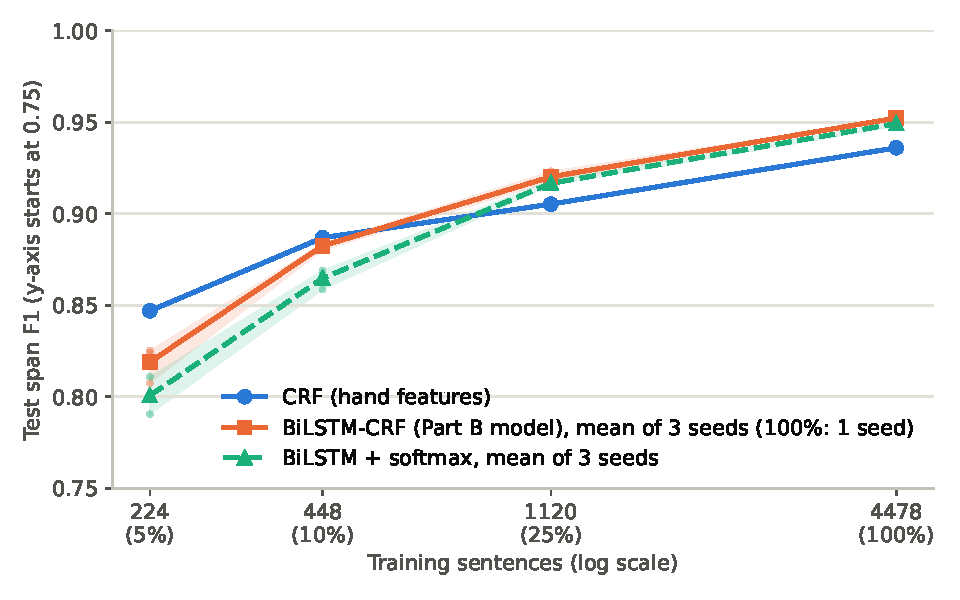
\includegraphics[width=\linewidth]{figures/data_efficiency.pdf}
\caption{Test span F1 vs.\ training-set size (log scale). BiLSTM curves are the
mean of 3 seeds at 5--25\% (band = min--max, dots = individual seeds; $\pm$ in
Table~\ref{tab:curve} is half that range) and 1 seed at 100\%. CRF training is
deterministic. The plotted BiLSTM uses a constant learning rate chosen on dev,
replacing a ReduceLROnPlateau schedule that undertrained the small subsets
(test F1 \oldLstmTestFive\ at 5\%, \oldLstmTestFull\ at 100\%).}
\label{fig:curve}
\end{figure}

\begin{table}[t]
\centering\small
\caption{Span F1 behind Fig.~\ref{fig:curve}. $\pm$ is half the min--max range over
3 seeds. Best test score per row in bold.}
\label{tab:curve}
\resizebox{\linewidth}{!}{\begin{tabular}{@{}rr ccc c@{}}
\toprule
 & & \multicolumn{3}{c}{Test span F1} & Dev span F1 \\
\cmidrule(lr){3-5}\cmidrule(l){6-6}
Frac. & Sent. & CRF & BiLSTM-CRF & BiLSTM+softmax & CRF / BiLSTM-CRF \\
\midrule
5\% & 224 & \textbf{0.847} & 0.819\,{\scriptsize$\pm$0.009} & 0.801\,{\scriptsize$\pm$0.010} & 0.853 / 0.848 \\
10\% & 448 & \textbf{0.887} & 0.882\,{\scriptsize$\pm$0.002} & 0.865\,{\scriptsize$\pm$0.005} & 0.891 / 0.899 \\
25\% & 1,120 & 0.905 & \textbf{0.920}\,{\scriptsize$\pm$0.003} & 0.917\,{\scriptsize$\pm$0.001} & 0.925 / 0.949 \\
100\% & 4,478 & 0.936 & \textbf{0.952} & 0.949\,{\scriptsize$\pm$0.001} & 0.954 / 0.979 \\
\bottomrule
\end{tabular}
}
\end{table}

\todo{Crossover discussion (graded: ``crossover discussed''). Where do the curves
cross, and why is each model ahead on its side of the crossover? Facts: on test
the CRF leads at 5\% (\crfTestFive\ vs \lstmTestFive) and 10\% (\crfTestTen\ vs
\lstmTestTen); the BiLSTM-CRF leads at 25\% (\lstmTestTwentyFive\ vs
\crfTestTwentyFive) and 100\% (\lstmTestFull\ vs \crfTestFull). On dev the
crossover is earlier (10\%: \crfDevTenFrac\ vs \lstmDevTen).}

\todo{What the CRF output layer buys the BiLSTM: compare BiLSTM-CRF and
BiLSTM+softmax across sizes (5\%: \lstmTestFive\ vs \smTestFive; 100\%:
\lstmTestFull\ vs \smTestFull).}

\todo{Honesty notes, 1--2 sentences: single CRF run per point (deterministic);
3 seeds for small BiLSTM runs. An earlier BiLSTM recipe with ReduceLROnPlateau
under-trained the small-data runs (old test F1 at 5\%: \oldLstmTestFive; 100\%:
\oldLstmTestFull); switching to a constant lr was chosen on dev and moved the
crossover.}

On test the curves cross between 10\% and 25\% of the training data.
The CRF leads at \nSentFive\ sentences (\crfTestFive\ vs.\ \lstmTestFive) and at
\nSentTen\ (\crfTestTen\ vs.\ \lstmTestTen); the BiLSTM-CRF leads at
\nSentTwentyFive\ (\lstmTestTwentyFive\ vs.\ \crfTestTwentyFive) and at
\nSentFull\ (\lstmTestFull\ vs.\ \crfTestFull).
Dev flips earlier, at \nSentTen\ (\lstmDevTen\ vs.\ \crfDevTenFrac).
Below the crossover, gazetteers, shape, and the $\pm1$ templates already supply
regularities the randomly initialized encoder has not learned: the
\lstmTestFive\ $\pm 0.011$ band stays under \crfTestFive.
Above it, the encoder covers dependencies outside that window, such as a verb
several tokens from its time.
On dev, switching from ReduceLROnPlateau to the constant learning rate moves
the crossover from between 10\% and 25\% to between 5\% and 10\%.
On test both schedules still cross between 10\% and 25\%. The constant rate
shrinks the 10\% test gap from 0.028 (\crfTestTen\ vs.\ \oldLstmTestTen) to
0.004 (\crfTestTen\ vs.\ \lstmTestTen). Full-data test F1 barely changes
(\oldLstmTestFull\ to \lstmTestFull).

The CRF output layer is worth the most while the encoder is weak:
\lstmTestFive\ vs.\ \smTestFive\ at 5\%, where the transition matrix blocks
illegal BIO paths. The two heads tie at 25\% (\lstmTestTwentyFive\ and
\smTestTwentyFive) and the full-data gap is \lstmTestFull\ vs.\ \smTestFull.
The win over the feature CRF is the encoder. The structured output is a
small-data constraint.

% =====================================================================
\section{Part D: Error analysis}
\begin{table}[t]
\centering\small
\caption{Test-set error profile of the two 100\% models.}
\label{tab:errsum}
\resizebox{\linewidth}{!}{\begin{tabular}{@{}lrr@{}}
\toprule
Span errors on test (2,837 gold spans) & CRF & BiLSTM-CRF \\
\midrule
wrong type & 142 & 102 \\
wrong boundary & 12 & 11 \\
type + boundary & 8 & 7 \\
missed & 33 & 21 \\
spurious & 6 & 10 \\
\midrule
recall, spans w/ OOV token (n=50) & 0.540 & 0.620 \\
recall, in-vocab spans (n=2787) & 0.938 & 0.956 \\
\midrule
sentences wrong (this model only) & 53 & 29 \\
sentences wrong for both & \multicolumn{2}{c}{87} \\
\bottomrule
\end{tabular}
}
\end{table}

\begin{table}[t]
\centering\small
\caption{Slot types ($n\ge5$) with the largest F1 gap.}
\label{tab:perslot}
\resizebox{\linewidth}{!}{\begin{tabular}{@{}lrrrr@{}}
\toprule
Slot type & $n$ & CRF & BiLSTM-CRF & $\Delta$ \\
\midrule
\texttt{aircraft\_code} & 33 & 0.935 & 0.653 & -0.282 \\
\texttt{fromloc.airport\_code} & 5 & 0.909 & 0.769 & -0.140 \\
\texttt{arrive\_time.start\_time} & 8 & 0.750 & 0.941 & +0.191 \\
\texttt{arrive\_time.time} & 34 & 0.746 & 0.943 & +0.197 \\
\texttt{airport\_code} & 9 & 0.200 & 0.444 & +0.244 \\
\texttt{arrive\_date.month\_name} & 6 & 0.286 & 0.769 & +0.484 \\
\texttt{arrive\_date.day\_number} & 6 & 0.286 & 0.769 & +0.484 \\
\texttt{arrive\_time.end\_time} & 8 & 0.200 & 0.800 & +0.600 \\
\texttt{arrive\_date.day\_name} & 11 & 0.235 & 0.880 & +0.645 \\
\texttt{arrive\_time.period\_of\_day} & 6 & 0.000 & 0.857 & +0.857 \\
\bottomrule
\end{tabular}
}
\end{table}

% Factual notes you can use (not conclusions):
% D1 (176): "arrives" is token 9, "950" is token 14 (5 positions away); CRF sees full features at +-1, words only at +-2.
% D2 (368): "l1011" is OOV; CRF shape = xdddd; BiLSTM sees <UNK> between "an" and "aircraft".
% D3/D4 (359, 512): "phl", "tpa" OOV and not in the airport-code gazetteer; whole utterance is "what is X".
% D5 (204): gold tags "india" as O (speaker restart before "indianapolis"); "india" is OOV.
% D6 (773): "757" is in train vocab, "hold" is OOV; CRF has isdigit/shape features on "757".
% D7/D8 (164, 165): "320", "dh8" OOV, both right after "aircraft".
% D9 (51): gold treats "665 673" as one flight_number span.
% D10 (243): "be1" OOV after airline name "delta".

\todo{One diagnosis per example, contrasted across models. The rubric wants the
mechanism, e.g.\ ``CRF misses unseen city names because word-identity features
can't fire''. Suggested grouping below; merge or reorder freely.}

\todo{Tie back to the aggregates: Table~\ref{tab:errsum} (most errors are
wrong-type, not boundary; recall on spans containing an OOV token is
\crfOovRecall\ for CRF vs \lstmOovRecall\ for BiLSTM, over \oovSpans\ spans) and
Table~\ref{tab:perslot} (which slot families each model owns).}

Most remaining errors are the wrong type: 142 for the CRF and 102 for the
BiLSTM-CRF, against 12 and 11 boundary errors (Table~\ref{tab:errsum}).
The models find the span and then assign the wrong role, the same gap $\pm1$
context closed in the feature log (\crfRoleIdentity\ role errors down to
\crfRoleCtxOne). The BiLSTM-CRF misses fewer spans (21 vs.\ 33).
The CRF alone is wrong on \nCrfWrongOnly\ sentences, the BiLSTM-CRF alone on
\nLstmWrongOnly, and both on \nBothWrong.
Recall on spans with an unseen token is \crfOovRecall\ vs.\ \lstmOovRecall\
(\oovSpans\ spans), against 0.938 and 0.956 in vocabulary.
The CRF leads on \slot{aircraft_code} (0.935 vs.\ 0.653, $n{=}33$) from word
identity, digit/shape, and the word ``aircraft'' beside the code. There is no
aircraft-code gazetteer. It also leads on \slot{fromloc.airport_code}
(0.909 vs.\ 0.769, $n{=}5$), where the airport-code list can fire.
The BiLSTM-CRF leads on bare \slot{airport_code} (0.444 vs.\ 0.200, $n{=}9$)
and on compositional time and date roles, including
\slot{arrive_time.period_of_day} (0.857 vs.\ 0.000, $n{=}6$).
The period list contains ``morning'' and ``evening,'' and the CRF's F1 on that
slot is still zero: the list marks a period, and the arrive/depart role is left
to context.

\textbf{Errors only the CRF makes (D1--D4).}

\textbf{D1.} Gold and the BiLSTM-CRF mark ``950 am'' as \slot{arrive_time.time};
the CRF emits \slot{depart_time.time}.
The time regex fires on the unseen digits and ``am'' is in the period list, but
``arrives'' (token 9) is five positions from ``950'' (token 14), outside the
$\pm1$ template and the $\pm2$ words.
The BiLSTM's state at the time still contains the verb.

\textbf{D2.} Gold and the BiLSTM-CRF mark unseen ``l1011'' as \slot{aircraft_code};
the CRF emits nothing.
Shape \texttt{xdddd} sets neither \texttt{isdigit} nor the time regex, and
there is no aircraft-code list.
The BiLSTM sees \texttt{<UNK>} between ``an'' and ``aircraft'' and labels it
from that frame.

\textbf{D3 and D4.} ``phl'' and ``tpa'' are unseen and absent from the
airport-code list, which keeps only codes from training.
Gold is \slot{airport_code}. The BiLSTM-CRF gets both, since both map to
\texttt{<UNK>} in ``what is \texttt{<UNK>}.''
The CRF has no identity feature and no list hit, so it misses both.

\textbf{Errors only the BiLSTM makes (D5--D8).}

\textbf{D5.} Gold leaves unseen ``india'' as O, a restart before
``indianapolis.'' The city list does not contain ``india,'' so the CRF also
emits O.
The BiLSTM sees \texttt{<UNK>} after ``from'' and emits \slot{fromloc.city_name}.

\textbf{D6.} ``757'' is in the training vocabulary; ``hold'' is unseen.
Gold and the CRF mark a one-token \slot{aircraft_code}, from word identity and
\texttt{isdigit}.
The BiLSTM pulls \texttt{<UNK>} into the span and emits \slot{transport_type}
on ``757 hold.''

\textbf{D7 and D8.} Unseen ``320'' and ``dh8'' sit immediately after ``aircraft.''
Gold and the CRF mark \slot{aircraft_code} from that previous-word feature; the
BiLSTM sees \texttt{<UNK>} and emits O.
This is the reverse of D2, and it is why \slot{aircraft_code} is the CRF's
largest gap in Table~\ref{tab:perslot}.

\textbf{Errors both make (D9--D10).}

\textbf{D9.} Gold is one \slot{flight_number} span on unseen ``665 673.''
The CRF emits two spans, one per digit string, and the BiLSTM keeps only ``665.''
\texttt{isdigit} and the time regex fire on each token separately, so neither
model joins the unseen pair.

\textbf{D10.} Gold is \slot{airline_name} on ``delta'' and \slot{aircraft_code}
on unseen ``be1.''
The CRF merges ``delta be1'' into one airline span.
The BiLSTM splits them and labels ``be1'' as \slot{flight_number}, the usual
short code after an airline name.

% =====================================================================
\section{Would I have switched to neural in 2014?}
\todo{One paragraph, knowing only what this assignment showed. At what data size?
Consider: the crossover point, the cost of feature engineering vs.\ the cost of
tuning (the lr-schedule episode), seed variance, and what the error analysis says
each model is good at.}

With only these results, I would ship the BiLSTM-CRF on the full training set
and keep the linear CRF below the test crossover, between \nSentTen\ and
\nSentTwentyFive\ sentences.
At \nSentFull\ the neural model leads \lstmTestFull\ to \crfTestFull, 1.6
points. That is the scale of the last two feature steps on dev, from
\crfDevCtxOne\ to \crfDevFull\ (2.6 points). The $\pm1$ context step, 0.782 to
\crfDevCtxOne, was 14.6 points.
The gain is uneven: long-range roles and compositional dates and times, plus
OOV recall \lstmOovRecall\ vs.\ \crfOovRecall, while \slot{aircraft_code} stays
with the CRF (0.935 vs.\ 0.653) via identity, shape, and the word ``aircraft.''
The constant learning rate had to be chosen on dev, where it does move the
crossover. On test it does not, and the old schedule was already ahead at full
data (\oldLstmTestFull). The 5\% seed band is about a point. I would have
shipped the BiLSTM-CRF at \nSentFull\ after locking that learning rate, and
left the feature CRF in place for equipment codes and for the small side of the
test crossover.
Mesnil et al.\ (2015) made that comparison for ATIS: recurrent taggers
passing a CRF \cite{mesnil2015}.

\begingroup
\footnotesize
\setlength{\itemsep}{0pt}
\begin{thebibliography}{1}
\bibitem{mesnil2015}
Mesnil, G., Dauphin, Y., Yao, K., Bengio, Y., Deng, L., Hakkani-Tur, D.,
He, X., Heck, L., Tur, G., Yu, D., and Zweig, G. 2015.
Using recurrent neural networks for slot filling in spoken language understanding.
\textit{IEEE/ACM Transactions on Audio, Speech, and Language Processing},
23(3):530--539.
\end{thebibliography}
\endgroup

\clearpage
\appendix
% The disclosure starts on its own page so it is easy to see it is outside the 3-page body.
\section*{AI-use disclosure}
% Draft list of what an AI assistant did, from the session log. Verify, edit,
% and add anything else you used AI for.
\todo{Name the tools and versions you used.}
\begin{itemize}
  \item \todo{What you wrote yourself and what AI wrote (e.g.\ boilerplate in
  \texttt{train.py}, \texttt{models/}, helper scripts).}
  \item Code review: an AI assistant (Claude) compared the repo with the course
  skeleton, simulated the autograder's inference check on the submission zip, and
  checked the Viterbi decoder and CRF loss against brute-force enumeration.
  \item Experiments run by the assistant at my request: the CRF feature ablation
  (\texttt{crf\_ablation.py}), removing two test-only airport codes from the
  gazetteer and retraining the CRF, extra BiLSTM seeds, the softmax-only BiLSTM
  (\texttt{--no-crf}), and the constant-lr BiLSTM recipe that replaced the
  submitted checkpoint after it scored higher on dev.
\end{itemize}

\end{document}
